\pagebreak
\section{Architectural Design}
 
\subsection{High level components}
According to the requirements described in RASD, we decided to design the architecture depicted
in Figure~\ref{fig:h_l_comp} and Figure~\ref{fig:i_h_l_comp}. These two figures represents
only a high level description of the components. In the first one we decided to focus on
the somewhat physical representation of our application. By saying physical we mean that
every component depicted there, will probably reside on separate machines (or is an external service).
To be precise we should have added another component between clients and
application server which is the reverse proxy/web server. The reason why we preferred to
omit it is that at this stage we want to address only the aspects that are relevant to the
application development and that layer can be considered quite transparent, the application
does not have to deal with it explicitly. Of course this will not be the same in a context of deployment.
The second figure instead is a high level overview of the application internals without all
the external components. We are going to describe its architecture further in this document
but we wanted nonetheless to give an initial idea of how it is internally structured.

We can summarize the two main aspects of our architecture in: client-server and microservices.

\subsubsection{Client-Server}
The architecture of the complete system will be a client-server one. We think this is the
most natural (if not only) way to build a distributed application supporting different
client technologies (mobile app, web app, etc.).

\subsubsection{Microservices}
Internally the application will be structured as a service oriented architecture.
More specifically we will try to build microservices that will deal with single, atomic, responsibilities.
\pagebreak

\begin{sidewaysfigure}
\centering
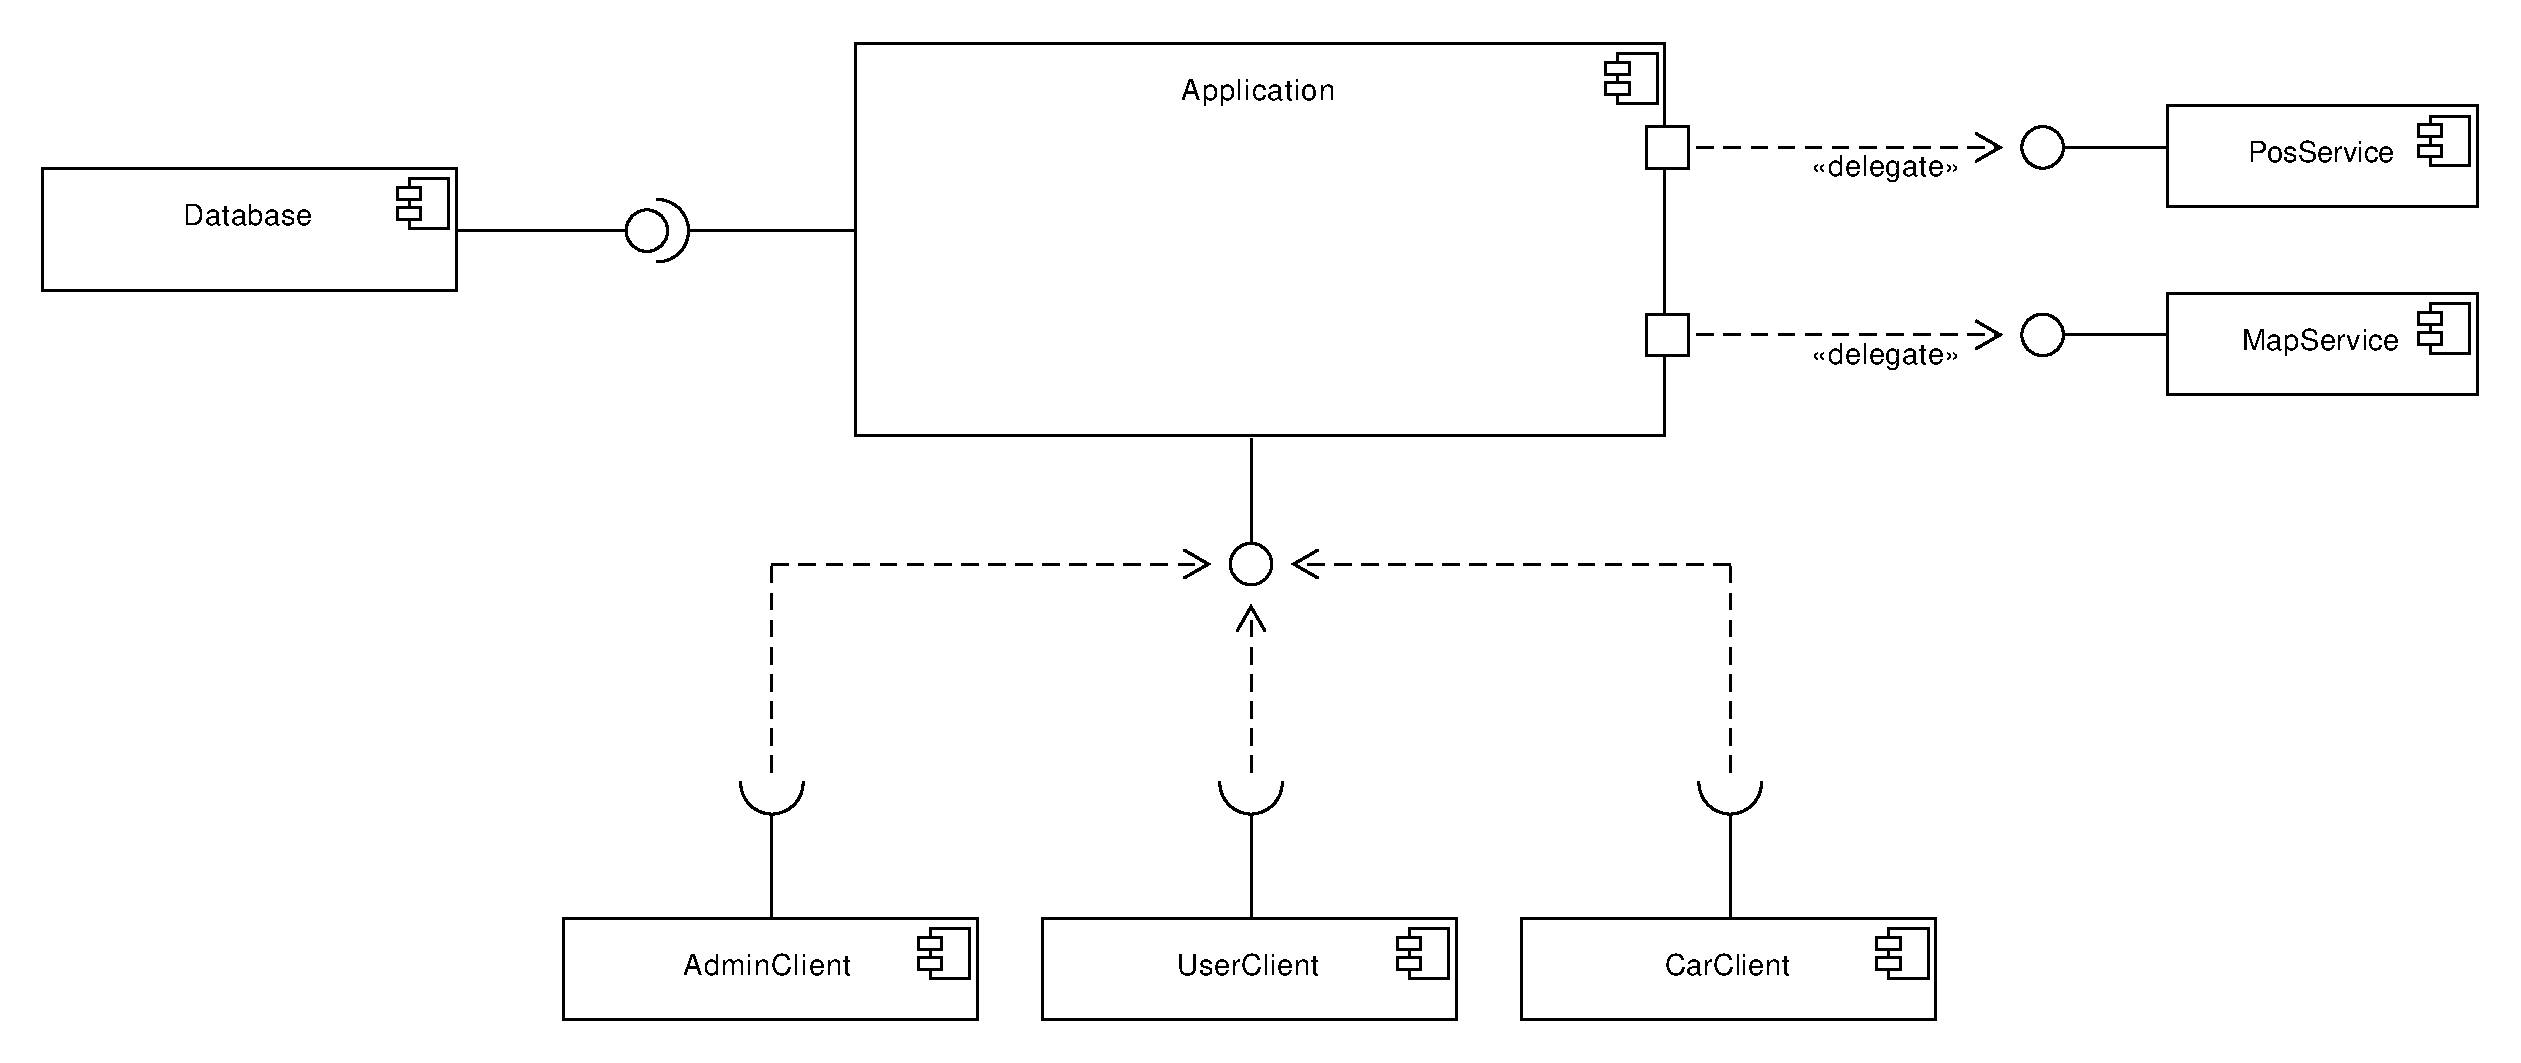
\includegraphics[width=\textwidth]{high_level_components}
\caption{Component view: High Level Architecture}
\label{fig:h_l_comp}
\end{sidewaysfigure}

\pagebreak

\begin{sidewaysfigure}
\centering
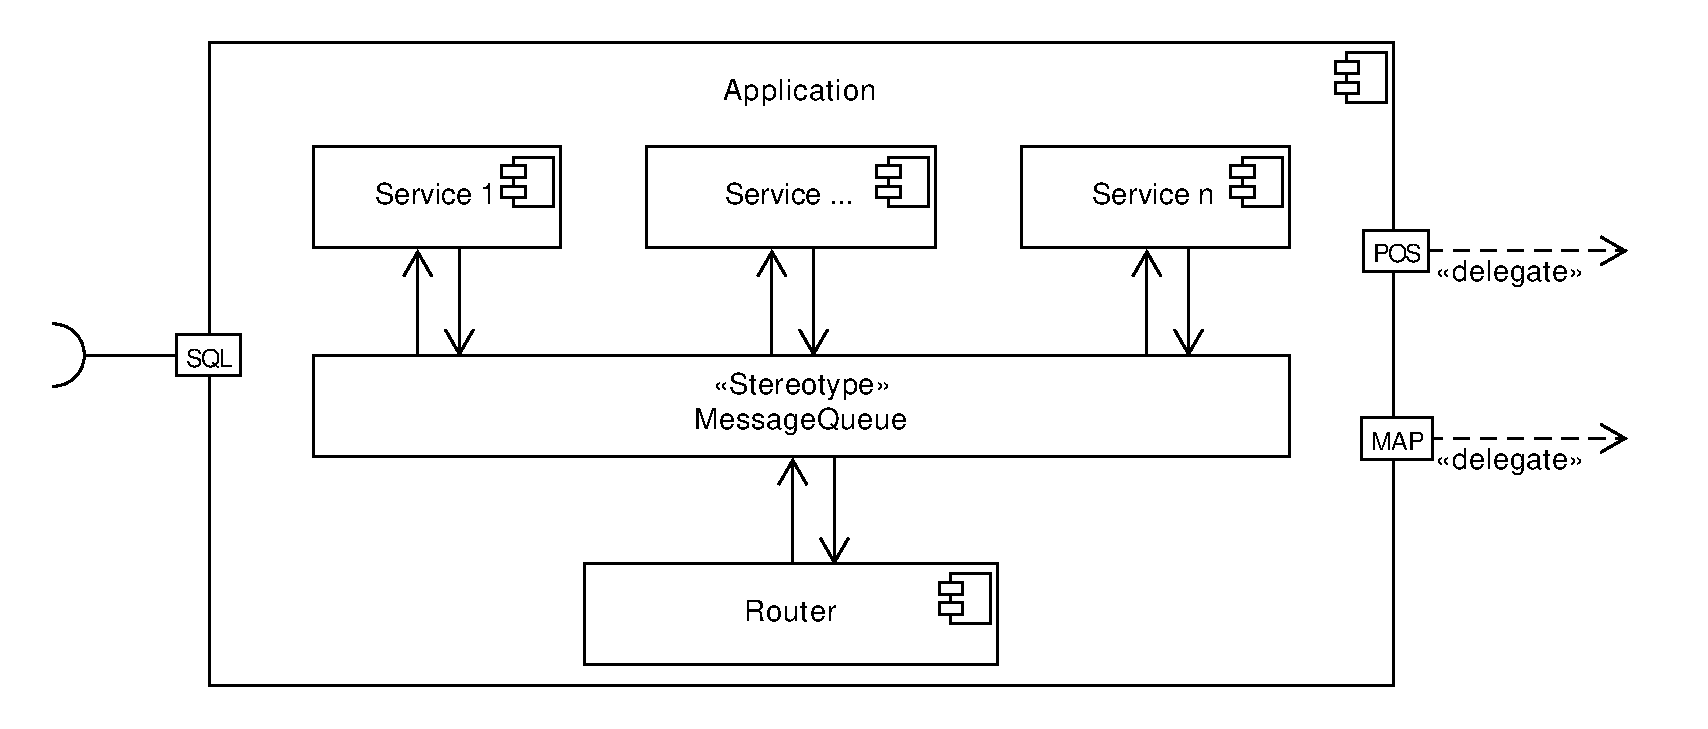
\includegraphics[width=\textwidth]{internal_high_level_components}
\caption{Component view: Internal High Level Architecture}
\label{fig:i_h_l_comp}
\end{sidewaysfigure}

\pagebreak

\begin{sidewaysfigure}
\centering
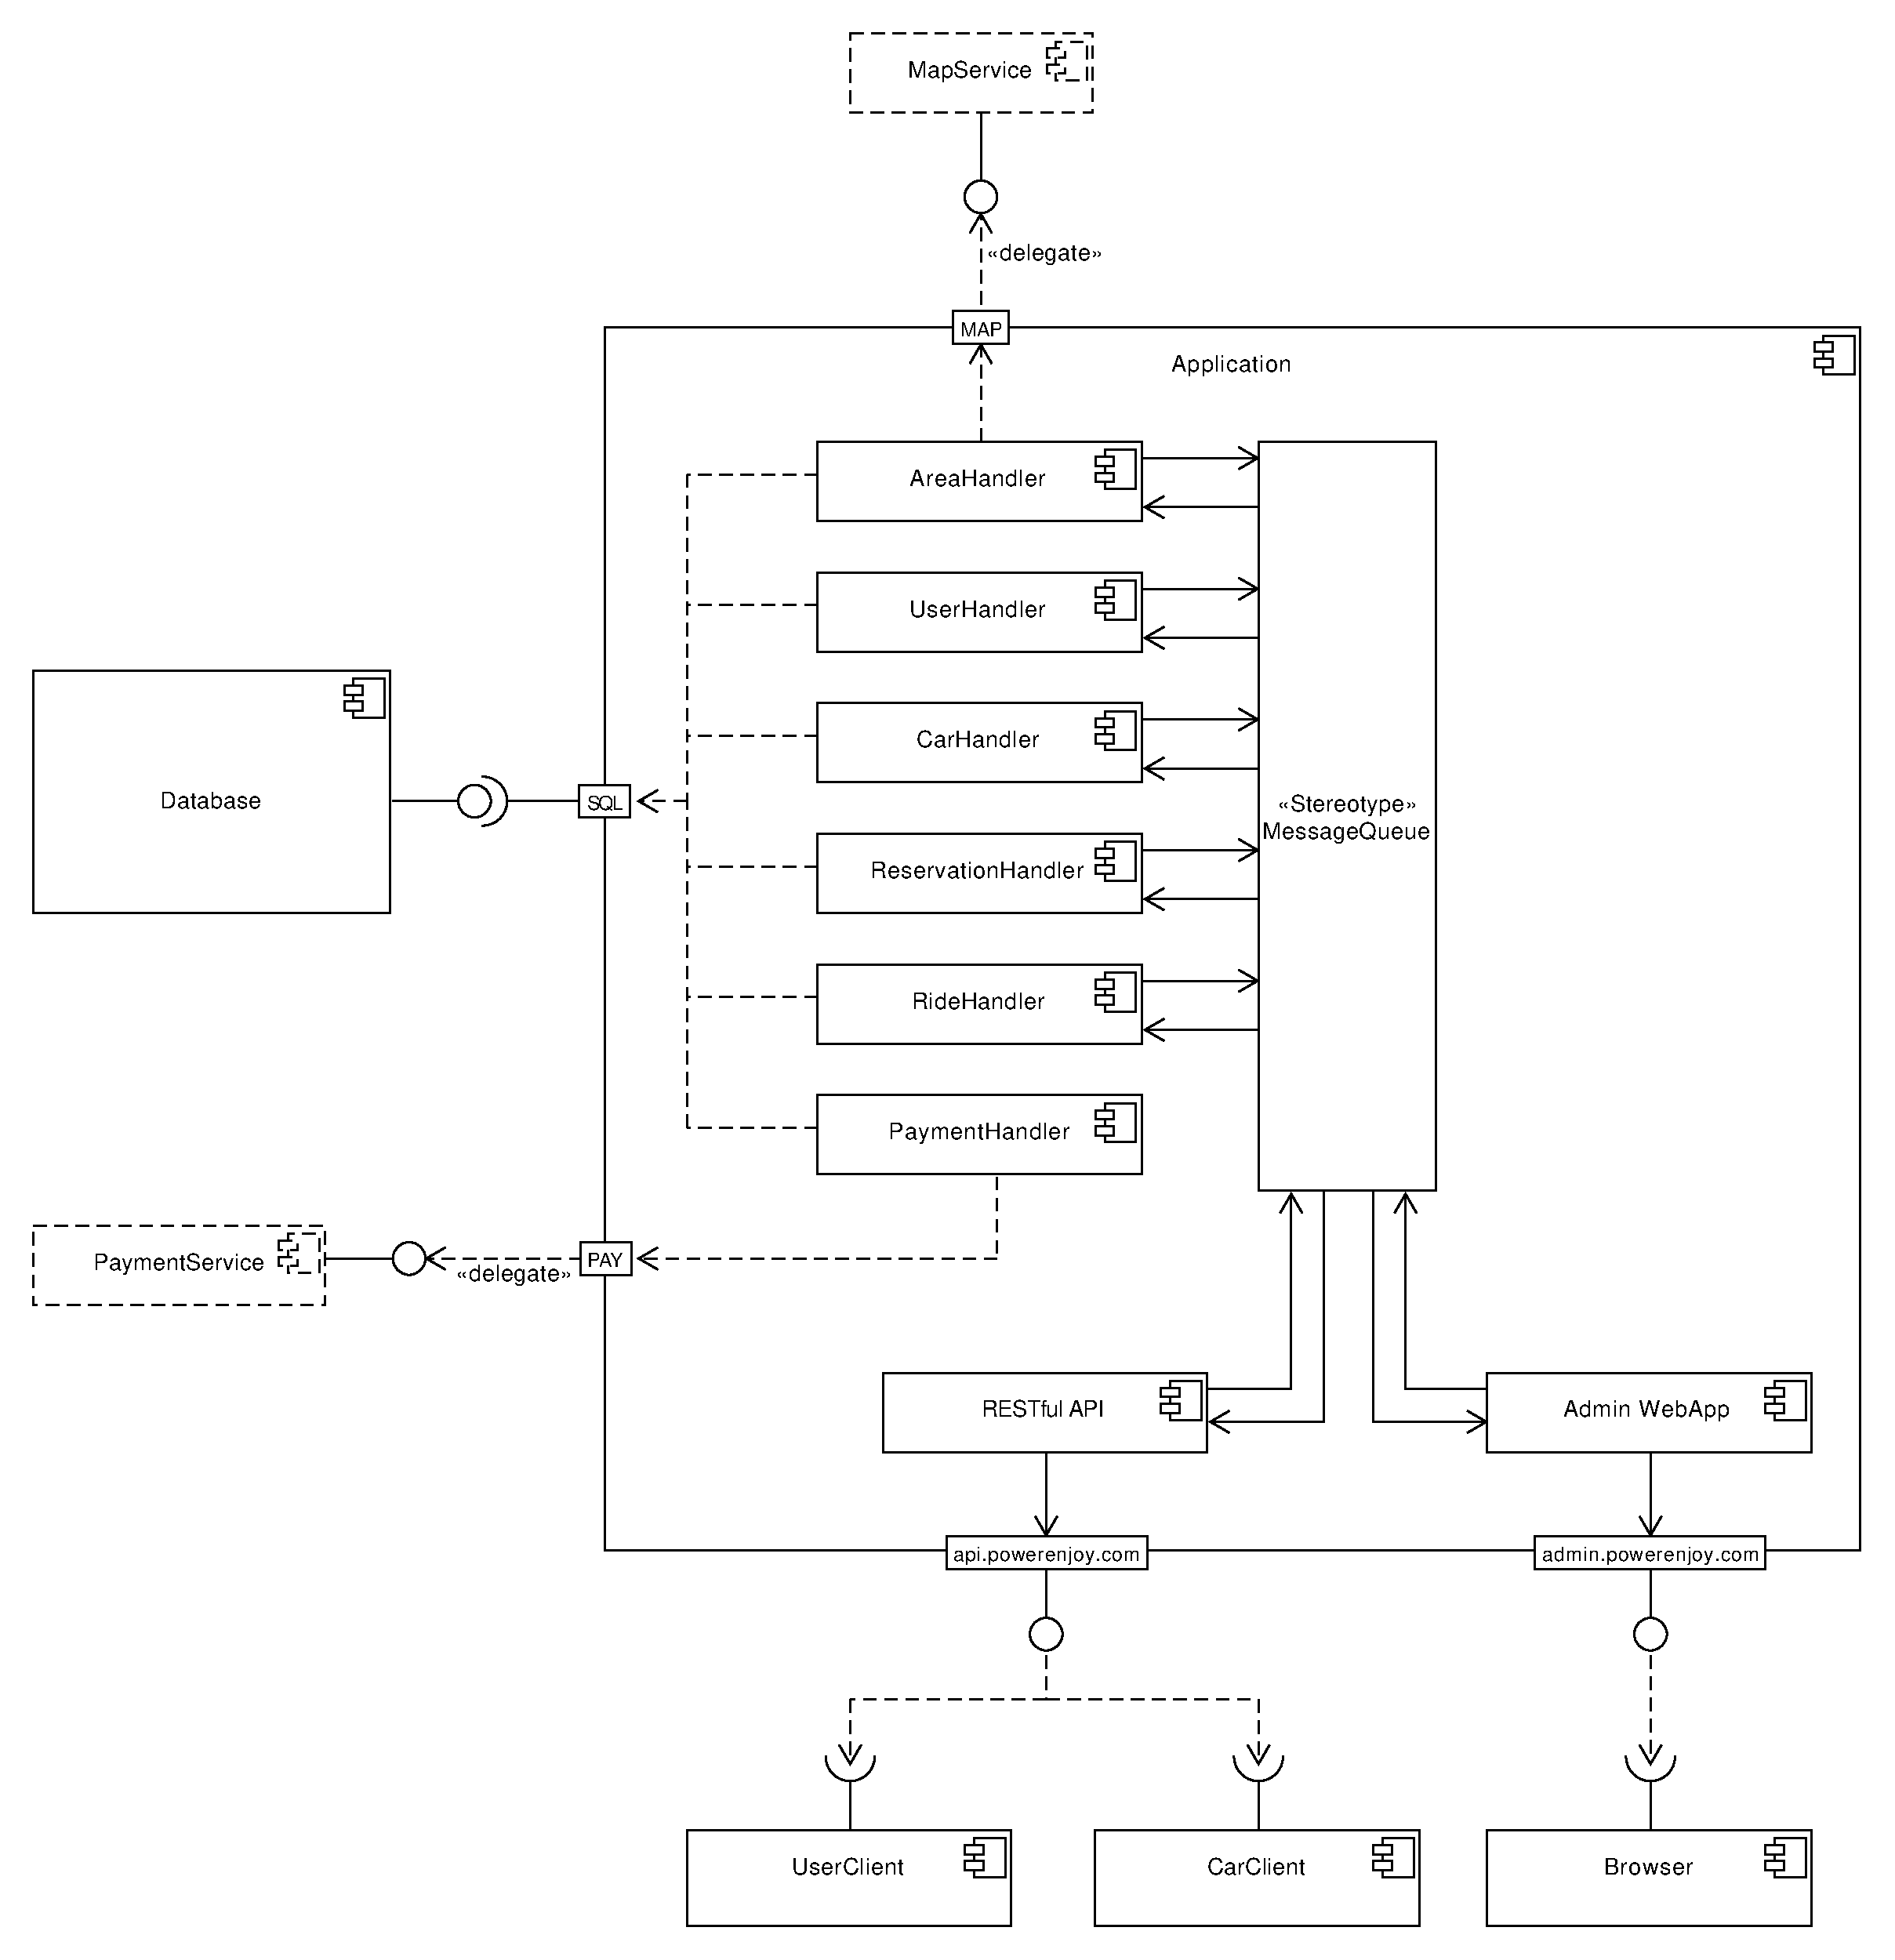
\includegraphics[width=\textwidth]{low_level_components}
\caption{Component view: Internal Low Level Architecture}
\label{fig:i_l_l_comp}
\end{sidewaysfigure}

\pagebreak
